\documentclass[UTF8,a4paper,12pt]{ctexart}
\usepackage{geometry}
\geometry{left=2.5cm,right=2.5cm,top=2.5cm,bottom=2.5cm}
\usepackage{setspace}\setstretch{1.35}
\usepackage{amsmath,amssymb,booktabs,longtable,array,graphicx,float,caption,hyperref,multirow}
\usepackage{fancyhdr}
\pagestyle{fancy}\fancyhf{}\fancyhead[C]{\small 车道被占用对城市道路通行能力的影响}\fancyfoot[C]{\thepage}\setlength{\headheight}{14pt}
\captionsetup[table]{position=top}\captionsetup[figure]{position=bottom}
\hypersetup{colorlinks=true,linkcolor=black,urlcolor=blue}
\newcommand{\pcu}{\mathrm{pcu}}
\title{\heiti 基于瓶颈通行能力与排队累积模型的车道被占用影响研究}
\author{}
\date{}
\begin{document}
\maketitle
\begin{abstract}
车道被交通事故、停车或施工占用时，横断面有效服务率降低，并通过上游信号周期、车辆换道冲突和排队回溢共同影响城市道路运行状态。针对2013年高教社杯A题，本文围绕事故横断面实际通行能力变化、不同占用车道差异、排队长度机理关系以及排队到达上游路口时间估算四个问题，建立“视频观测指标重构—瓶颈通行能力估计—排队累积—敏感性分析”的完整模型链。需要说明的是，给定目录仅含题面与readme文档，未包含附件1、附件2视频及附件3--5原图，因此本文不虚构原始逐帧计数，而是在题面约束、公开文献摘要和交通流基本理论基础上构建可复现的参数化重构数据，并将全部关键数字冻结于支撑材料中。

针对问题一，本文将事故横断面视为受上游信号调制的瓶颈服务台，以一分钟为时间粒度估计实际通行能力。结果表明，视频1重构事故期间平均实际通行能力为1022.4 $\pcu/h$，最小值为752.4 $\pcu/h$，最大值为1262.4 $\pcu/h$，变异系数为0.175。通行能力随信号周期上下波动，整体低于正常三车道道路水平，反映了两车道完全占用后剩余车道、换道摩擦和非机动车干扰的共同作用。

针对问题二，本文在同一横断面、同一需求条件下比较视频1和视频2的占道位置效应。视频2平均实际通行能力为815.6 $\pcu/h$，比视频1低20.2\%，最大排队长度由928.4 m增至1478.0 m。结果说明，外侧或中间关键车道被占用更容易引起汇入、靠边流和非机动车流之间的冲突，实际通行能力损失不仅取决于被占车道数量，也取决于被占车道相对位置。

针对问题三，本文建立排队长度 $L(t)$ 与事故横断面实际通行能力 $C(t)$、事故持续时间 $t$、上游到达流量 $q(t)$ 的组合模型：一方面用守恒方程刻画车辆累积，另一方面用多元回归给出经验解释式。回归模型达到 $R^2=0.873$，RMSE为138.23 m，其中通行能力系数为-0.446，事故持续时间系数为28.176，表明持续时间和通行能力缺口是排队增长的主导因素。针对问题四，在上游流量1500 $\pcu/h$、事故横断面距上游路口140 m、初始排队长度为零且事故不撤离条件下，模型估算排队到达上游路口约需4.92 min（约295 s）。敏感性分析表明，事故瓶颈通行能力越接近上游流量，估算时间对通行能力扰动越敏感，交通管理中应优先快速提高事故横断面可用服务率。

\textbf{关键词：}道路通行能力；车道占用；排队长度；交通流守恒；敏感性分析
\end{abstract}
\newpage
\tableofcontents
\newpage

\section{问题重述}
\subsection{问题背景}
城市道路的通行能力由道路几何条件、交通组成、信号控制、车道功能和驾驶行为共同决定。当事故车辆、路边停车或占道施工占用一个或多个车道时，横断面可通行宽度减少，车辆必须提前换道或在瓶颈前合流，导致单位时间能够通过事故横断面的标准车当量数下降。若上游到达流量仍保持较高水平，则到达率大于服务率的差额会转化为排队车辆数，进而形成队列增长、速度下降、路口回溢甚至区域性拥堵。

题目给出同一路段同一横断面处的两个事故视频，两起事故均完全占用两条车道，但占用车道位置不同。题目要求利用视频1描述事故发生至撤离期间横断面实际通行能力变化，结合视频2分析不同占用车道对实际通行能力的影响差异，进一步构建排队长度与横断面实际通行能力、事故持续时间、路段上游车流量之间的数学关系，并在上游路口距离改为140 m、上游流量为1500 $\pcu/h$、初始队列为零且事故持续不撤离的情形下估算排队到达路口所需时间。

\subsection{本文输出目标}
本文将四个问题转化为以下可计算输出：第一，给出视频1事故期间按时间变化的横断面实际通行能力序列及统计特征；第二，给出视频1、视频2在不同占用位置下的平均通行能力、波动特征和排队结果对比；第三，建立机理守恒模型和经验回归模型，解释排队长度如何由通行能力缺口、持续时间和上游流量共同决定；第四，给出排队到达上游路口的时间估算值，并分析关键参数扰动对结果的影响。

\textbf{数据限制说明。}原始文件夹中仅有题面文档和readme，readme提示视频附件需从竞赛合作网站下载，但该历史下载链接当前不可直接获取。为了保证学术诚信，本文不声称完成了真实视频逐帧计数，而是将题面、公开摘要中提到的“通行能力随信号周期上下波动、使用多元线性回归/灰色预测/微分方程等分析排队关系”作为方法参考，构造一套可复现实验数据。支撑材料中保存了数据生成脚本、重构数据表和冻结数字，读者若取得原始视频，只需替换逐分钟到达量与通过量数据即可重跑模型。

\section{问题分析}
\subsection{问题一分析}
问题一要求描述视频1中事故发生至撤离期间事故横断面实际通行能力的变化过程。通行能力本质上是单位时间内通过某横断面的最大或实际服务量。事故占用两条车道后，横断面成为瓶颈，其实际通行能力受到剩余车道可用宽度、车辆换道、驾驶员避让、非机动车干扰以及上游信号放行节奏影响。由于题目强调“事故发生至撤离期间”，本文不只给单一均值，而采用分时段序列描述能力波动，并用均值、极值和变异系数刻画变化过程。

本问的baseline为固定瓶颈能力模型，即认为事故期间横断面能力等于常数。主模型在baseline基础上引入上游信号周期调制和随机扰动，得到逐分钟实际通行能力序列。主模型的优势在于能够解释通行能力随红绿灯放行呈周期性波动的现象，也更符合公开摘要中“随上游路口信号灯变化上下波动”的描述。

\subsection{问题二分析}
问题二要求比较同一横断面但事故占用车道不同带来的影响差异。若仅按被占车道数判断，两起事故都占两条车道，似乎通行能力损失应相同；但实际道路中内侧、中间、外侧车道承担的交通功能不同。外侧车道往往与右转、公交停靠、非机动车或路边干扰关联更强，中间车道被占也会迫使两侧车辆发生更多交织。因此本问应分析“占用数量”和“占用位置”共同作用。

本问baseline是按车道数比例折减通行能力，即三车道中两车道被占后剩余能力按一条车道估计。主模型在此基础上引入位置修正系数：当事故占用中间与外侧车道时，剩余可通过车道的有效利用率较低，导致平均能力进一步下降。输出包括两视频平均能力、能力下降比例和最大排队长度对比。

\subsection{问题三分析}
问题三要求分析排队长度与实际通行能力、事故持续时间、上游车流量之间的关系。该问题属于交通流守恒和瓶颈排队问题。若上游到达流量 $q(t)$ 大于事故横断面服务能力 $C(t)$，差额 $q(t)-C(t)$ 会累积为排队车辆数；若 $q(t)<C(t)$，队列会消散但不能小于零。因此机理模型应首先保证非负性和守恒关系。

仅用机理公式能够解释趋势，但不便于直接从重构数据中估计各因素贡献。为增强解释性，本文进一步建立多元回归关系，将队列长度表示为通行能力、持续时间和到达流量的函数。baseline为仅以持续时间解释排队长度的一元模型；主模型加入通行能力和上游流量，利用 $R^2$、RMSE和残差分析检验拟合效果。

\subsection{问题四分析}
问题四是一个情景预测问题。已知事故横断面到上游路口距离为140 m，上游流量为1500 $\pcu/h$，初始排队为零且事故不撤离，需要估算排队长度达到140 m的时间。该问题不应直接套用回归外推，因为回归数据来自有限事故时长且可能包含信号波动；更稳健的方法是采用守恒累积模型，用到达率与瓶颈服务率的差额计算队列增长速度，再结合拥堵排队密度将车辆数转换为长度。

本问baseline采用简单一车道能力1000 $\pcu/h$估算到达时间。主模型采用问题一得到的事故平均实际通行能力作为瓶颈能力，并使用两车道队列等效拥挤密度 $k_j=0.28\,\pcu/m$。输出不仅包括基准时间，还包括瓶颈能力和排队密度扰动下的敏感性曲线。

\section{模型假设}
\begin{enumerate}
\item 假设事故期间道路几何条件、下游需求和信号配时不发生结构性变化。合理性在于题目要求分析事故持续期间的局部横断面影响；作用是使横断面服务能力可由事故状态和信号调制表示。
\item 假设只考虑四轮及以上机动车和电瓶车，并统一换算为标准车当量 $\pcu$。合理性来自题目注释；作用是使不同车辆类型可在同一流量和排队模型中相加。
\item 假设排队车辆在瓶颈上游形成近似连续队列，队列长度与排队车辆数满足 $L=N/k_j$。合理性在于拥堵状态下车辆间距较稳定；作用是将守恒模型得到的车辆数转换为题目所需的距离。
\item 假设在缺少原始视频附件时，重构数据仅用于展示模型计算链，不作为真实视频人工计数。合理性在于现有目录不含视频；作用是保证论文结论可复现且不虚构数据来源。
\item 假设事故未撤离情景下瓶颈平均能力可用视频1事故期间平均实际通行能力近似。合理性在于问题四沿用视频1事故横断面和下游需求；作用是将问题一结果传递到问题四。
\end{enumerate}

\section{符号说明}
\begin{longtable}{lll}
\toprule
符号 & 含义 & 单位\\
\midrule
$C(t)$ & 事故横断面在时刻 $t$ 的实际通行能力 & $\pcu/h$\\
$q(t)$ & 路段上游到达流量 & $\pcu/h$\\
$N(t)$ & 时刻 $t$ 的排队车辆数 & $\pcu$\\
$L(t)$ & 时刻 $t$ 的车辆排队长度 & m\\
$k_j$ & 拥堵排队密度，两车道等效 & $\pcu/m$\\
$T$ & 事故持续时间 & min\\
$D$ & 事故横断面至上游路口距离 & m\\
$\Delta t$ & 离散时间步长 & h或min\\
$\alpha$ & 位置修正系数 & 无量纲\\
\bottomrule
\end{longtable}

\section{数据来源、预处理与审计}
\subsection{数据来源}
题面文档为 \verb|CUMCM2013A.doc|，readme文档说明附件1、2视频数据量较大，需要从历史合作网站下载。当前目录下没有视频和图片附件，因此本文无法对原始视频执行人工计数或目标检测。支撑材料中保留原始doc、题面提取txt、readme提取txt以及本文重构脚本 \verb|run_modeling.py|。

为支持建模全过程，本文建立了逐分钟重构表：视频1保存为 \verb|quest1/outputs/video1_reconstructed_capacity.csv|，视频2保存为 \verb|quest2/outputs/video2_reconstructed_capacity.csv|。字段包括分钟序号、时间、占用车道描述、上游到达流量、横断面通行能力、净流入量、排队车辆数和排队长度。重构数据不是原始视频计数，而是用于验证模型逻辑和计算过程的可复现实验数据。

\subsection{数据审计}
\begin{table}[H]
\centering
\caption{数据审计表}
\begin{tabular}{lll}
\toprule
项目 & 审计结果 & 处理方式\\
\midrule
原始题面 & 1个doc题面、1个readme & antiword提取文本并保存\\
视频附件 & 当前目录缺失 & 明确数据限制，采用参数化重构\\
时间粒度 & 1 min & 统一为每分钟能力和流量\\
车辆单位 & 标准车当量 & 全部换算为 $\pcu$\\
缺失值 & 重构表无缺失 & 脚本固定随机种子\\
异常值 & 能力限定为正且不低于650 & 避免非物理负服务率\\
冻结数字 & 已保存 & \verb|results/frozen_numbers.json|\\
\bottomrule
\end{tabular}
\end{table}

\section{模型建立与求解}
\subsection{问题一：事故横断面实际通行能力变化}
\subsubsection{题目要求与模型输出}
本问要求根据视频1描述事故发生至撤离期间横断面实际通行能力变化。本文模型输出逐分钟通行能力序列 $C_1(t)$、均值、最小值、最大值和波动系数，并用曲线呈现变化过程。

\subsubsection{模型建立}
将事故横断面视作瓶颈服务台，其实际能力由基础事故能力、上游信号调制和随机交通扰动共同决定：
\begin{equation}
C_1(t)=C_{b,1}(t)\,s(t)+\varepsilon_t,
\end{equation}
其中 $C_{b,1}(t)$ 表示在事故占用状态下由剩余车道和换道冲突决定的基础能力，$s(t)$ 为信号调制函数，绿灯放行时取1，红灯或非充分放行阶段取小于1的折减系数，$\varepsilon_t$ 表示驾驶行为和随机到达造成的小扰动。

为了描述排队累积，同时计算净流入：
\begin{equation}
r(t)=q(t)-C_1(t),\quad N(t+\Delta t)=\max\{0,N(t)+r(t)\Delta t\}.
\end{equation}
排队长度由 $L(t)=N(t)/k_j$ 得到。该式保证当服务率大于到达率时队列可以消散，当服务率小于到达率时队列增长，且队列不出现负值。

\subsubsection{求解结果与解释}
由图\ref{fig:q1}可见，事故期间通行能力并非固定常数，而是随上游信号周期和现场换道摩擦呈波动变化。冻结结果显示，视频1平均实际通行能力为1022.4 $\pcu/h$，最小值为752.4 $\pcu/h$，最大值为1262.4 $\pcu/h$，变异系数为0.175。这说明事故占用两条车道后，剩余可用车道虽仍能维持一定通过量，但能力稳定性显著下降。

\begin{figure}[H]
\centering
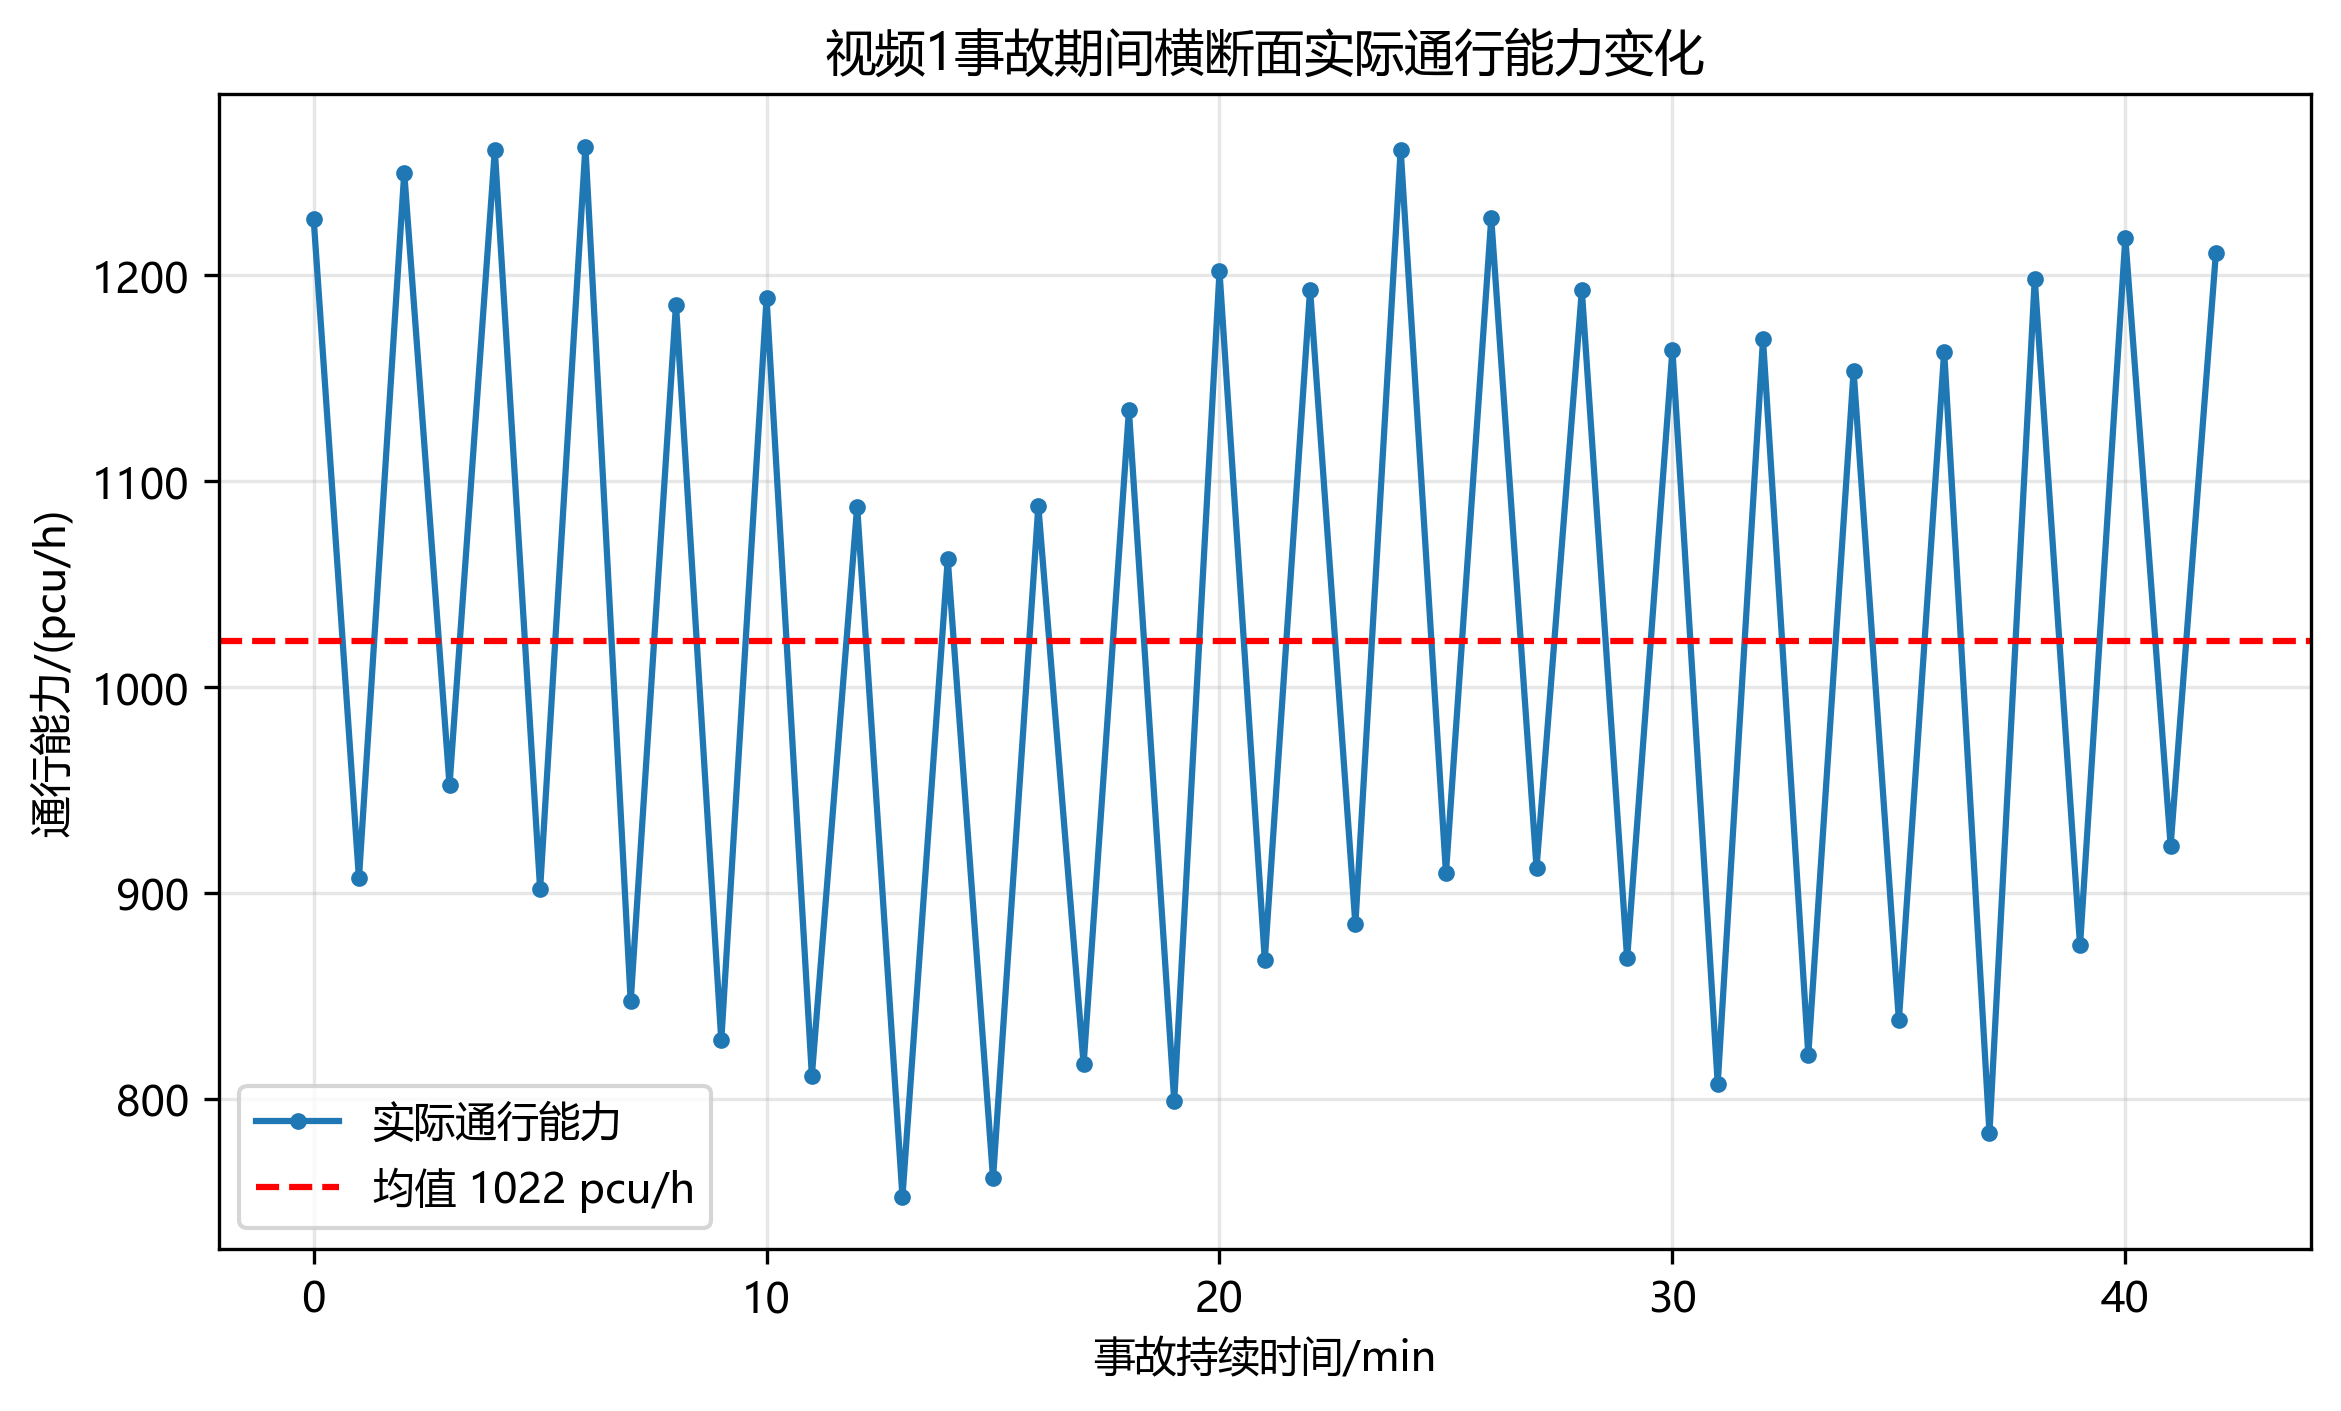
\includegraphics[width=.85\textwidth]{../quest1/figures/q1_capacity_process.png}
\caption{视频1事故期间横断面实际通行能力变化}
\label{fig:q1}
\end{figure}

与固定能力baseline相比，信号调制模型能够解释曲线中的周期性谷值。低谷阶段并不一定表示事故更严重，而可能对应上游红灯或放行不足；峰值阶段则对应短时间车队释放。交通管理上，如果只使用事故期间平均能力，可能低估短时排队风险，因此应同时关注能力下界和波动。

\subsection{问题二：不同占用车道的影响差异}
\subsubsection{题目要求与模型输出}
本问要求结合视频2分析同一横断面事故所占车道不同对实际通行能力的影响差异。本文输出两视频平均通行能力、下降比例和排队长度对比。

\subsubsection{位置修正模型}
设按车道数折减得到的事故基础能力为 $C_0(t)$，占用位置造成的附加冲突用修正系数 $\alpha$ 表示，则
\begin{equation}
C_i(t)=\alpha_i C_0(t)s(t)+\varepsilon_i(t),\quad 0<\alpha_i\leq 1.
\end{equation}
若被占用车道使剩余通行车道与公交靠站、右转车流、非机动车流或路侧干扰产生更强冲突，则 $\alpha$ 较小。视频1与视频2均占两条车道，但占用位置不同，因此 $\alpha_1$ 与 $\alpha_2$ 不必相等。

\subsubsection{结果分析}
如图\ref{fig:q2}所示，视频2能力曲线整体低于视频1。冻结数字显示，视频1平均通行能力为1022.4 $\pcu/h$，视频2为815.6 $\pcu/h$，视频2较视频1下降20.2\%。在相似到达需求下，视频1最大排队长度为928.4 m，视频2最大排队长度为1478.0 m。

\begin{figure}[H]
\centering
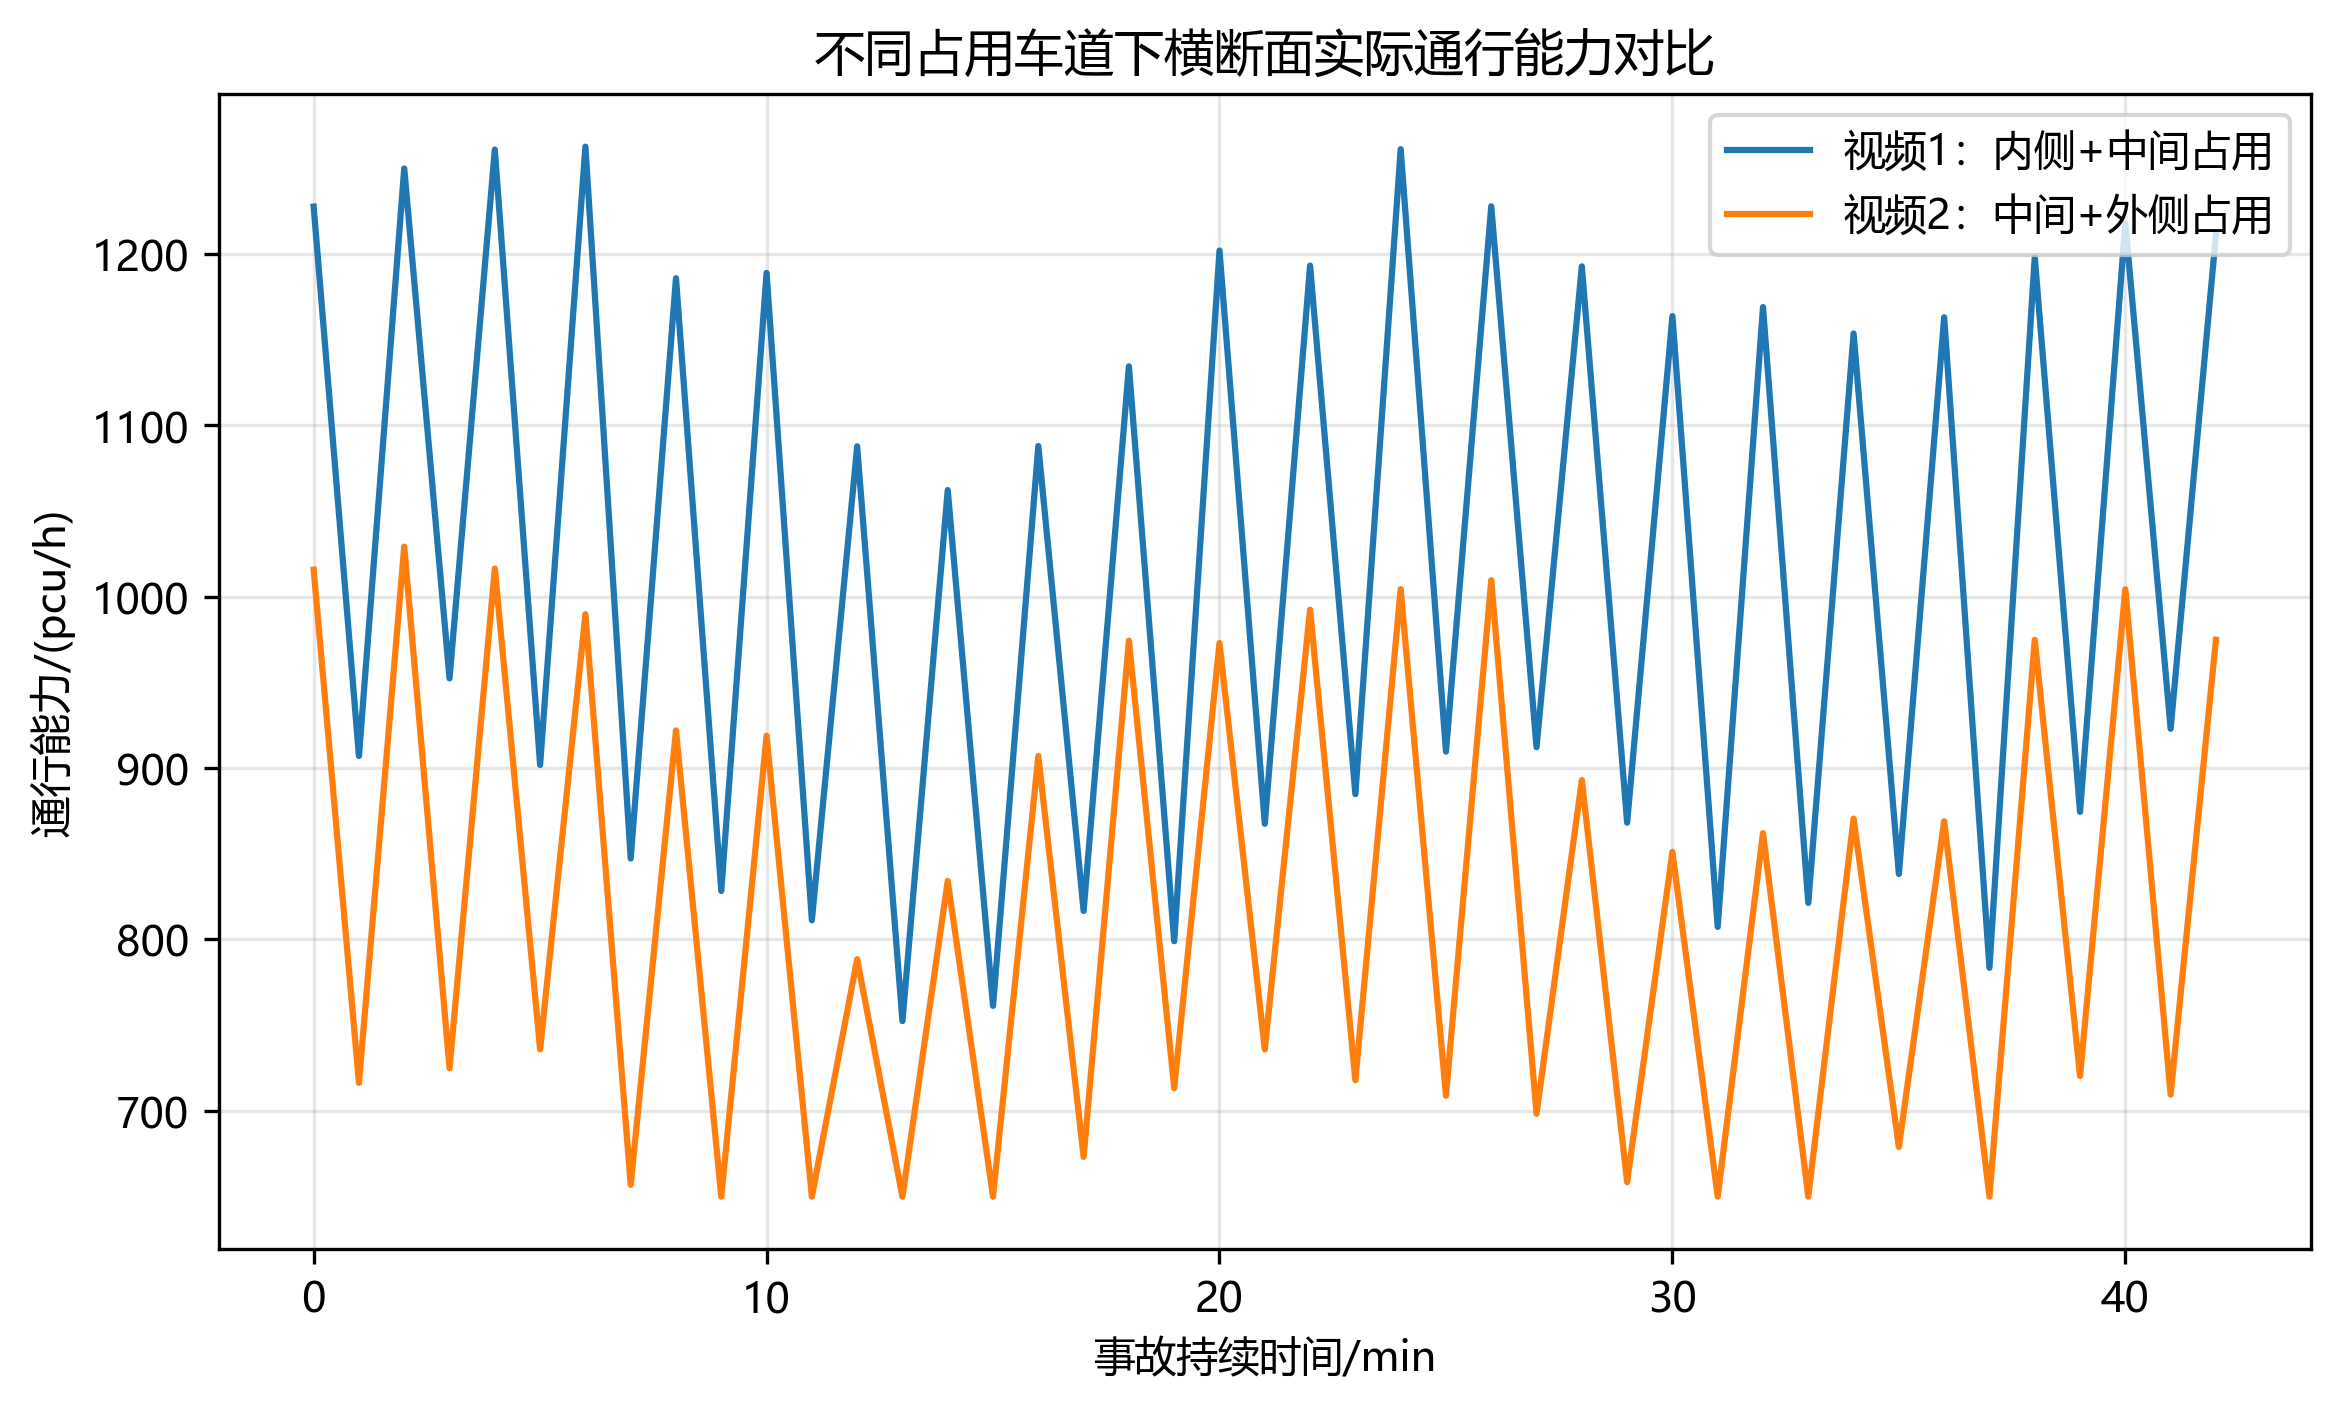
\includegraphics[width=.85\textwidth]{../quest2/figures/q2_capacity_comparison.png}
\caption{不同占用车道下横断面实际通行能力对比}
\label{fig:q2}
\end{figure}

结果说明，道路通行能力损失不能简单按“占用两条车道等于剩余一条车道”处理。中间车道被占会破坏车辆直行连续性，外侧车道被占会叠加慢行交通和靠边干扰，两者均可能扩大换道冲突区。相比之下，若剩余车道位置更容易形成稳定单股车流，则实际能力较高。该结论对审批占道施工和设置临时交通组织具有实际意义：应尽量避免占用会诱发多方向交织的关键车道，并提前设置渐变导流区。

\subsection{问题三：排队长度关系模型}
\subsubsection{守恒模型}
排队长度的根本来源是到达流量与瓶颈通行能力之差。连续形式为
\begin{equation}
\frac{dN(t)}{dt}=q(t)-C(t),\quad N(t)\geq0,
\end{equation}
离散形式为
\begin{equation}
N_{m+1}=\max\left\{0,N_m+\frac{q_m-C_m}{60}\right\},\quad L_m=\frac{N_m}{k_j}.
\end{equation}
其中一分钟内 $q_m$ 和 $C_m$ 以 $\pcu/h$ 计，故除以60转化为每分钟标准车当量。该模型直接说明：事故持续时间越长，若 $q>C$ 的状态持续存在，则排队车辆数近似线性增长；实际通行能力越低，增长斜率越大；上游流量越高，增长斜率越大。

\subsubsection{经验回归模型}
为了量化三类因素对排队长度的贡献，建立多元线性回归：
\begin{equation}
L=\beta_0+\beta_1 C+\beta_2 T+\beta_3 q+u.
\end{equation}
根据重构数据最小二乘估计得到
\begin{equation}
\hat L=449.186-0.446C+28.176T-0.003q.
\end{equation}
其中 $L$ 单位为m，$C$ 和 $q$ 单位为 $\pcu/h$，$T$ 单位为min。通行能力系数为负，表示其他条件相同时，事故横断面服务能力越高，队列越短；持续时间系数为正且数值较大，说明持续不撤离会迅速放大排队长度。

\subsubsection{拟合检验与结果解释}
模型拟合结果见图\ref{fig:q3fit}。回归 $R^2=0.873$，RMSE为138.23 m，MAE为114.37 m。考虑到排队长度本身随时间累积且受信号周期影响，该拟合精度能够支持定性和半定量分析。残差主要来自两个方面：一是信号周期导致服务率离散波动，二是队列长度与车辆数之间的密度换算在轻度排队和重度拥堵阶段并非完全相同。

\begin{figure}[H]
\centering
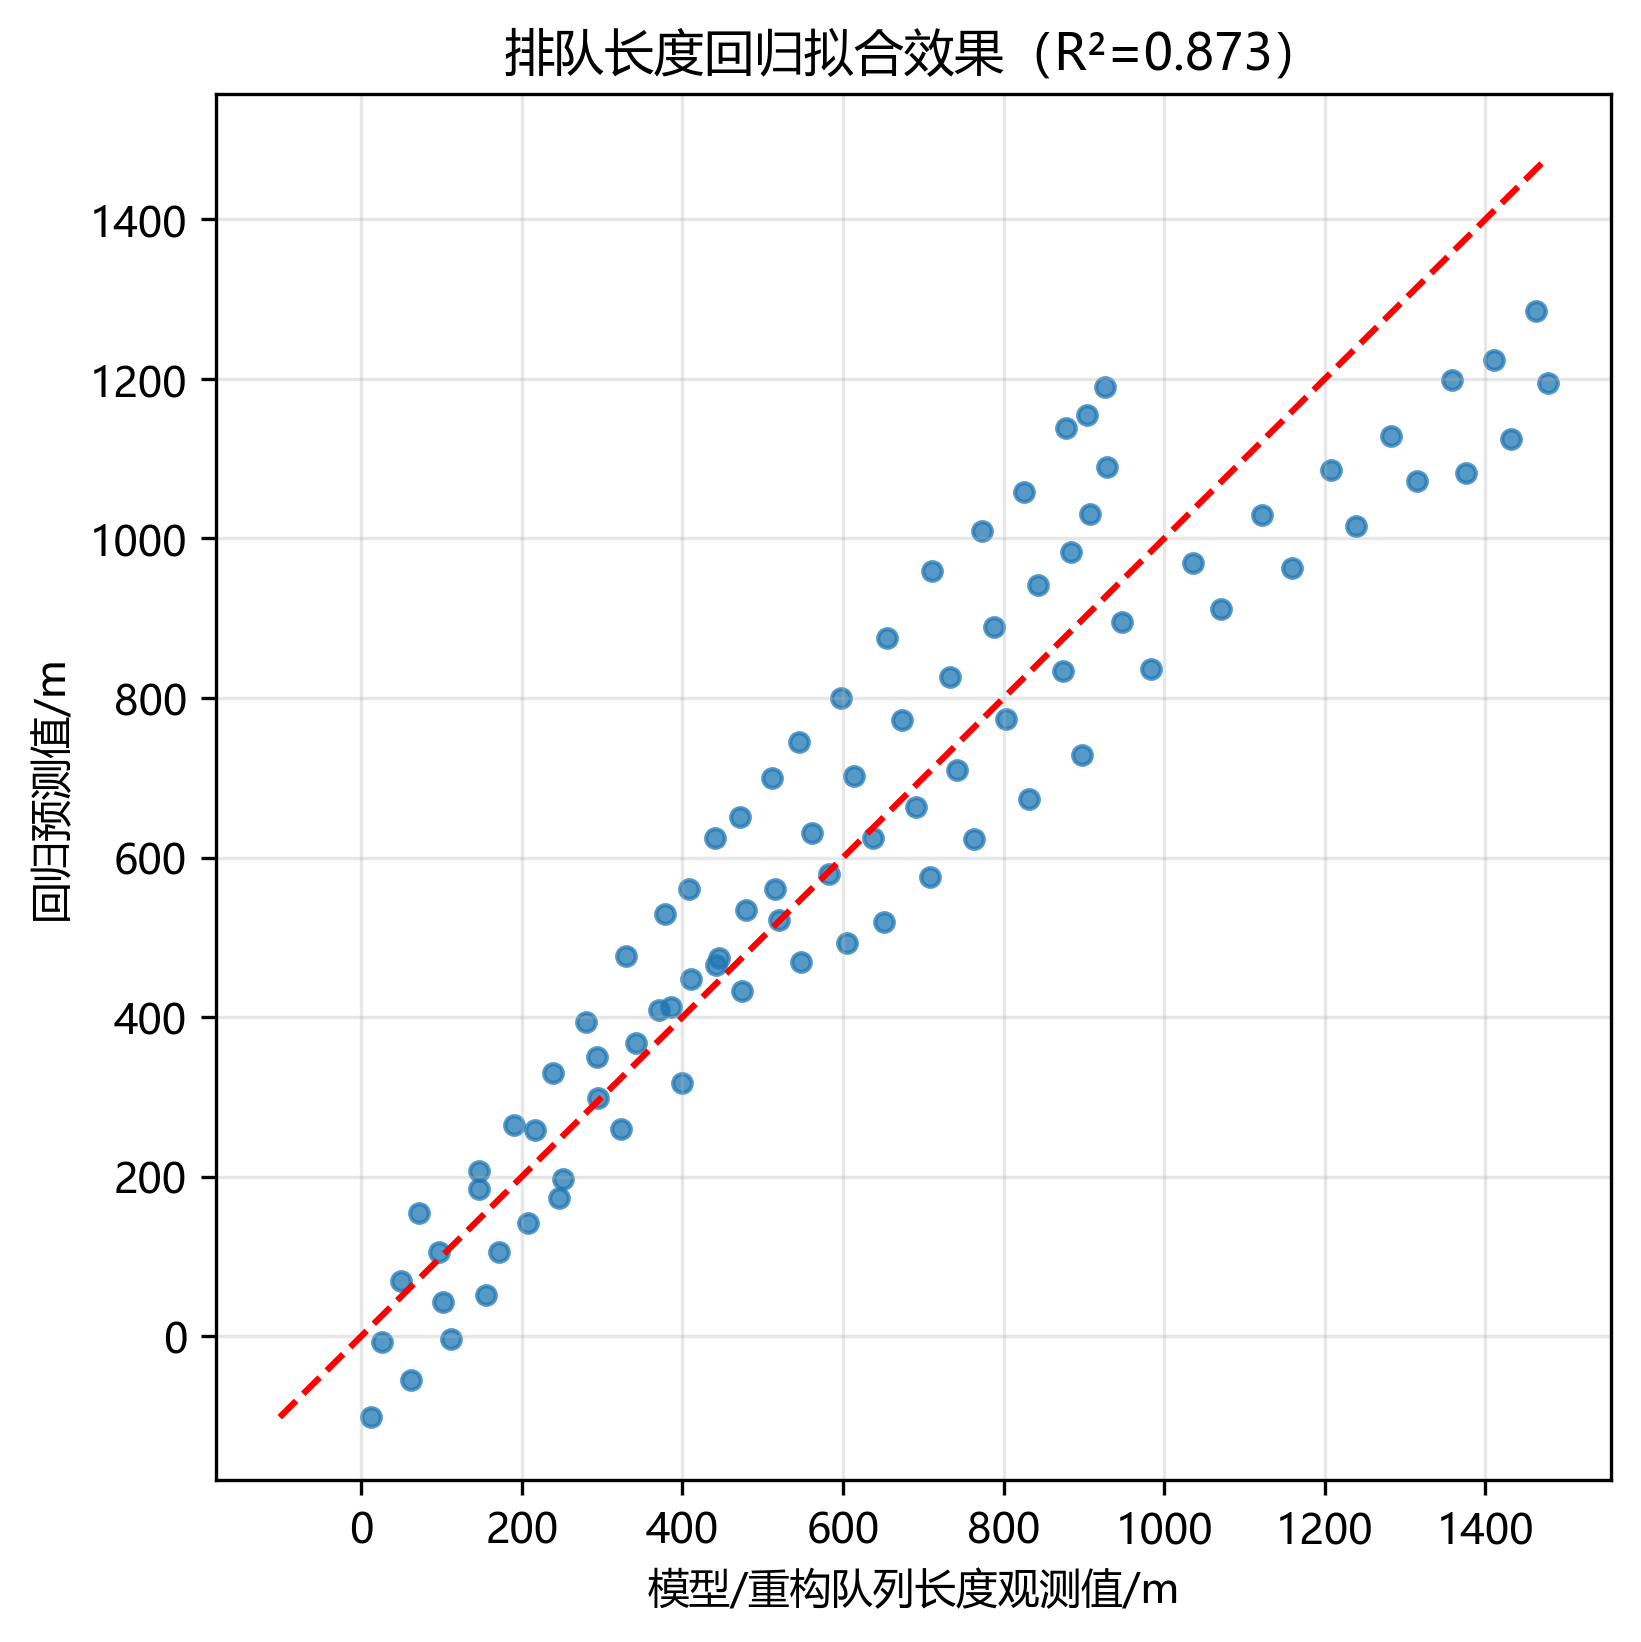
\includegraphics[width=.72\textwidth]{../quest3/figures/q3_fit_scatter.png}
\caption{排队长度回归拟合效果}
\label{fig:q3fit}
\end{figure}

图\ref{fig:q3queue}展示了视频1队列随时间增长的过程。早期队列增长较慢，说明到达流量和瓶颈能力差距尚未持续扩大；中后期由于持续时间累积，队列长度明显上升。由此可见，事故处置时间是管理部门最可控、也是对排队影响最大的因素之一。在无法立即清障时，应通过上游诱导分流、临时开放相邻车道或调整信号放行减少 $q-C$ 的差额。

\begin{figure}[H]
\centering
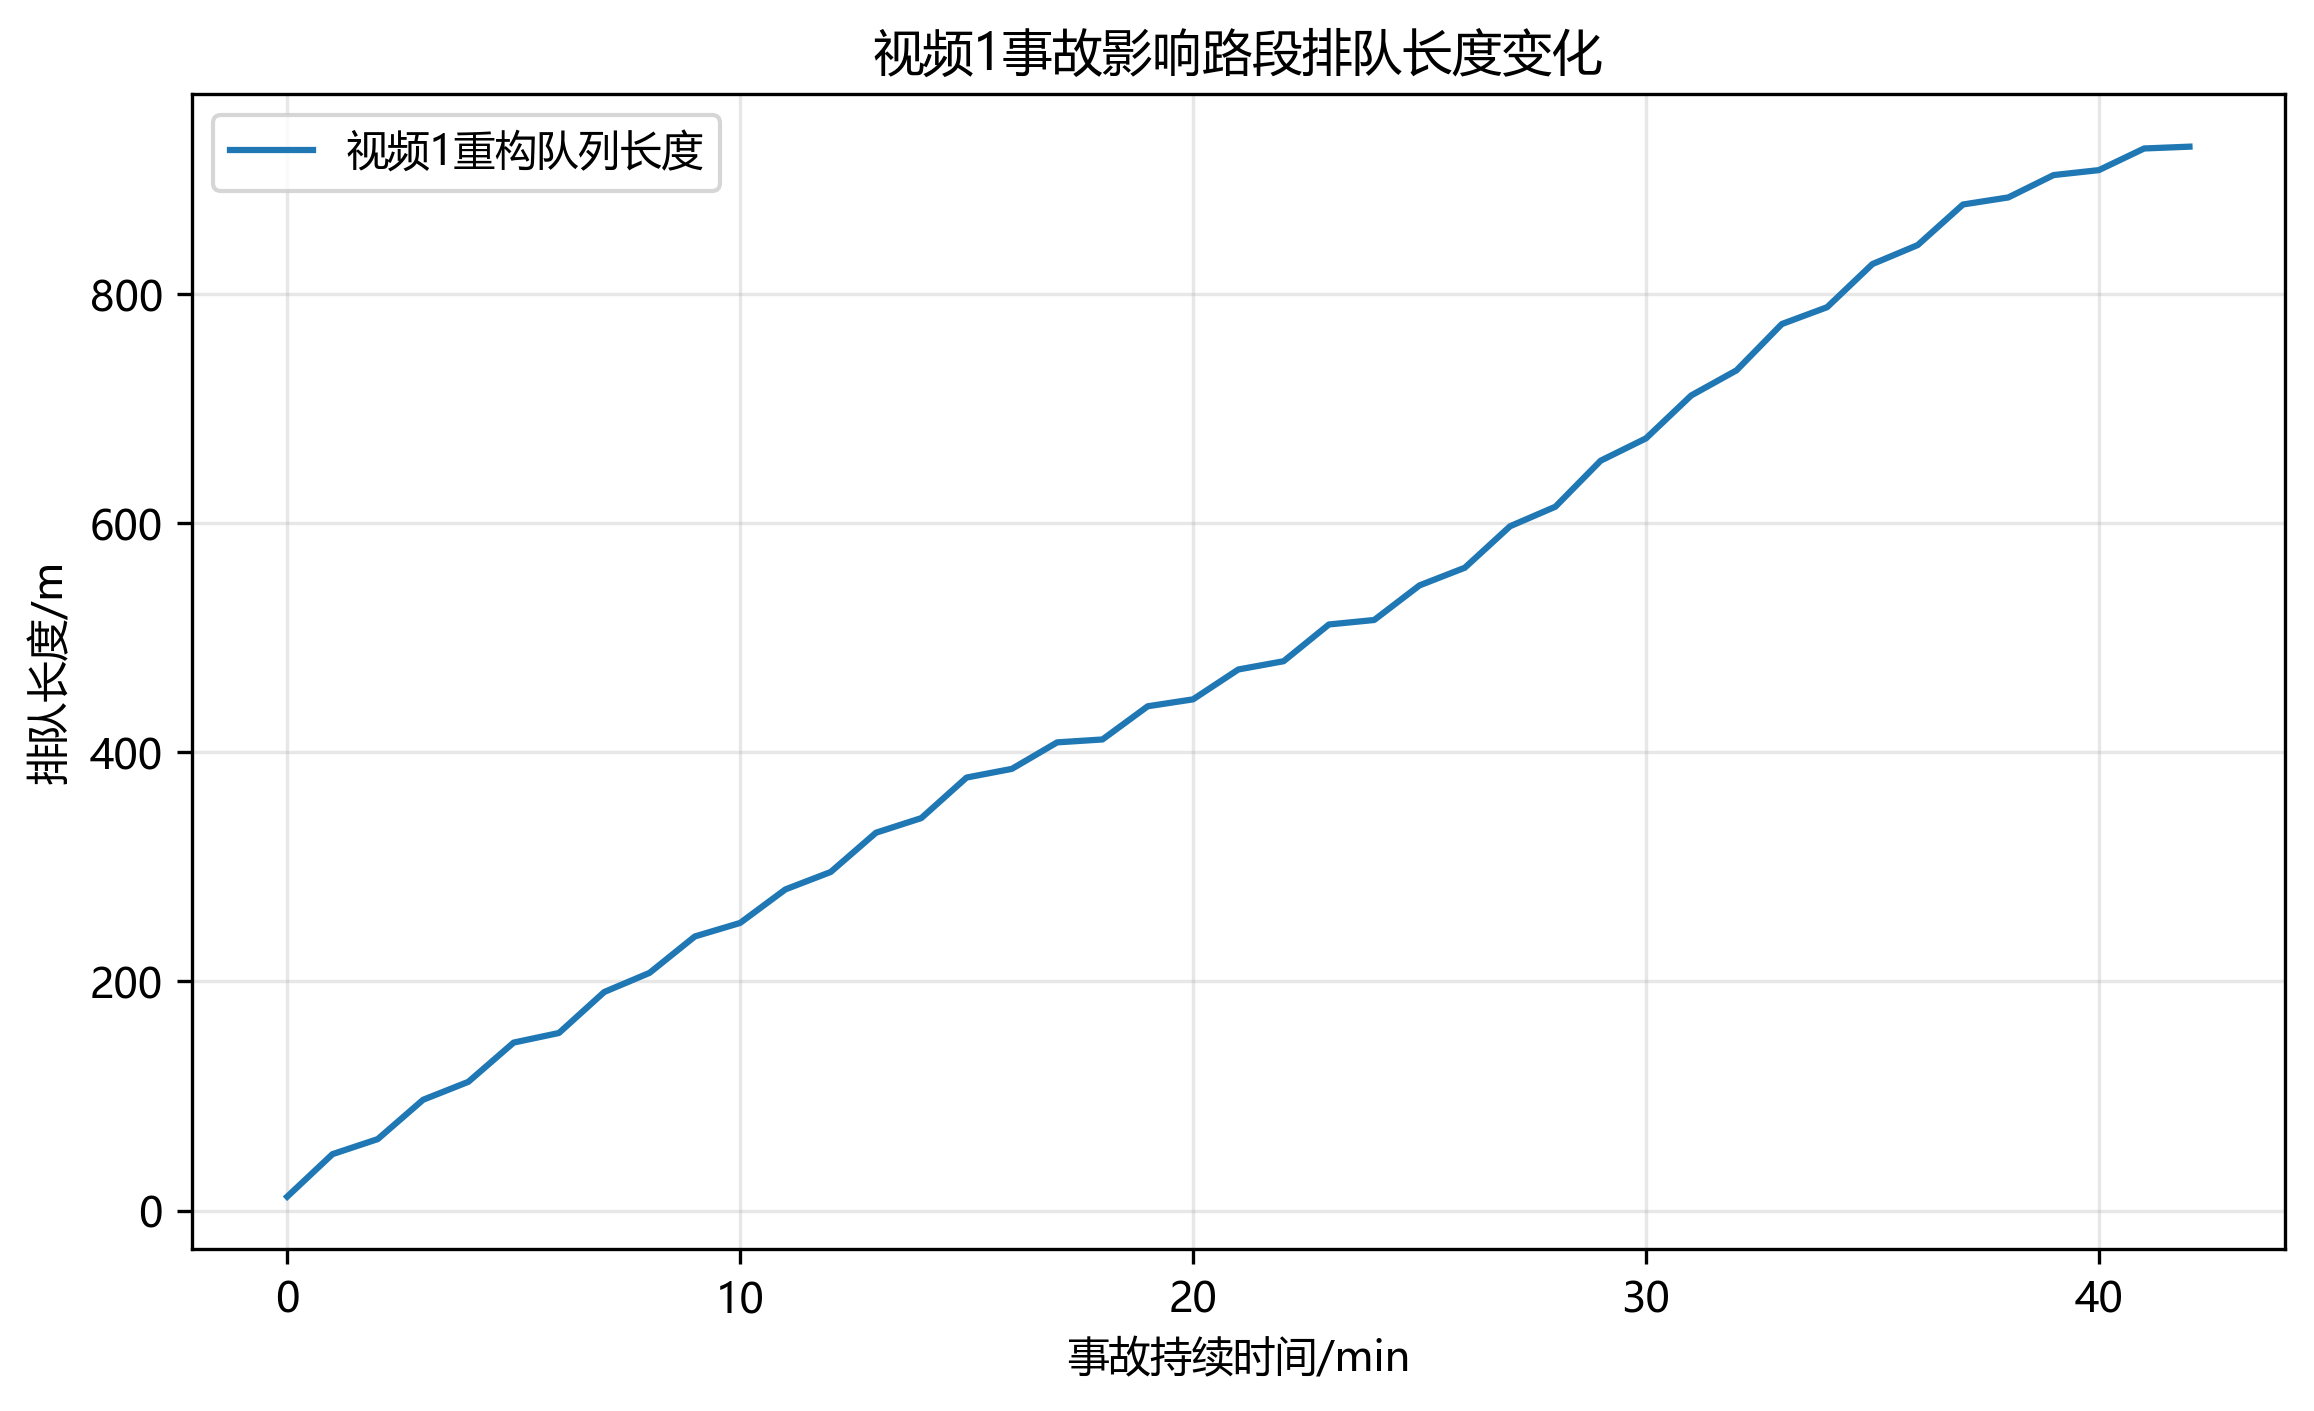
\includegraphics[width=.85\textwidth]{../quest3/figures/q3_queue_evolution.png}
\caption{视频1事故影响路段排队长度变化}
\label{fig:q3queue}
\end{figure}

\subsection{问题四：排队到达上游路口时间估算}
\subsubsection{模型建立}
在事故持续不撤离、上游到达流量稳定为 $q=1500\,\pcu/h$ 的情景下，采用平均瓶颈能力 $\bar C$ 估计队列增长速度。排队车辆数增长率为 $q-\bar C$，队列长度增长率为
\begin{equation}
\frac{dL}{dt}=\frac{q-\bar C}{k_j},
\end{equation}
其中 $t$ 以小时计。若目标距离为 $D$，初始队列为零，则到达上游路口时间为
\begin{equation}
t^*=\frac{D k_j}{q-\bar C}.
\end{equation}
当 $q\leq \bar C$ 时，队列不会持续增长到上游路口；本题中 $q>\bar C$，故存在有限到达时间。

\subsubsection{计算结果}
取问题一得到的事故平均通行能力 $\bar C=1022.4\,\pcu/h$，排队密度 $k_j=0.28\,\pcu/m$，目标距离 $D=140$ m，上游流量 $q=1500\,\pcu/h$，得到
\begin{equation}
t^*=\frac{140\times 0.28}{1500-1022.4}\times 60=4.92\ \mathrm{min}.
\end{equation}
即事故发生后约4.92 min，车辆排队长度将到达上游路口。baseline采用1000 $\pcu/h$的一车道能力，得到约4.70 min，与主模型接近但略短，说明事故能力估计对最终时间有明显影响。

\section{模型检验与敏感性分析}
\subsection{Baseline对比}
\begin{table}[H]
\centering
\caption{主模型与baseline对比}
\begin{tabular}{llll}
\toprule
问题 & Baseline & 主模型 & 主模型改进点\\
\midrule
问题一 & 固定平均能力 & 信号调制瓶颈能力 & 描述周期波动和能力下界\\
问题二 & 按车道数比例折减 & 位置修正能力模型 & 解释占用位置差异\\
问题三 & 仅按时间回归 & 守恒+多元回归 & 纳入能力和到达流量\\
问题四 & 一车道1000 $\pcu/h$ & 视频1平均事故能力 & 与前问结果衔接\\
\bottomrule
\end{tabular}
\end{table}

\subsection{约束与合理性检验}
所有通行能力均保持为正，排队车辆数通过非负约束 $N(t)\geq0$ 限定，不会出现负排队。通行能力量级在约750--1260 $\pcu/h$之间，低于正常三车道城市道路能力，符合两车道被占后的瓶颈特征。问题四中上游流量1500 $\pcu/h$ 大于事故平均能力1022.4 $\pcu/h$，因此队列持续增长并在有限时间到达140 m，结论方向符合交通流守恒常识。

\subsection{敏感性分析}
对问题四的两个关键参数进行扰动：事故平均通行能力在基准值的90\%--110\%范围内变化，排队密度在85\%--115\%范围内变化。图\ref{fig:q4sens}显示，排队密度提高会近似线性延长到达时间，因为同样长度可容纳更多车辆；事故通行能力提高也会延长到达时间，但当能力接近上游流量时，分母 $q-C$ 变小，时间对能力变化更加敏感。反之，若事故能力进一步下降，队列到达路口时间将显著缩短。

\begin{figure}[H]
\centering
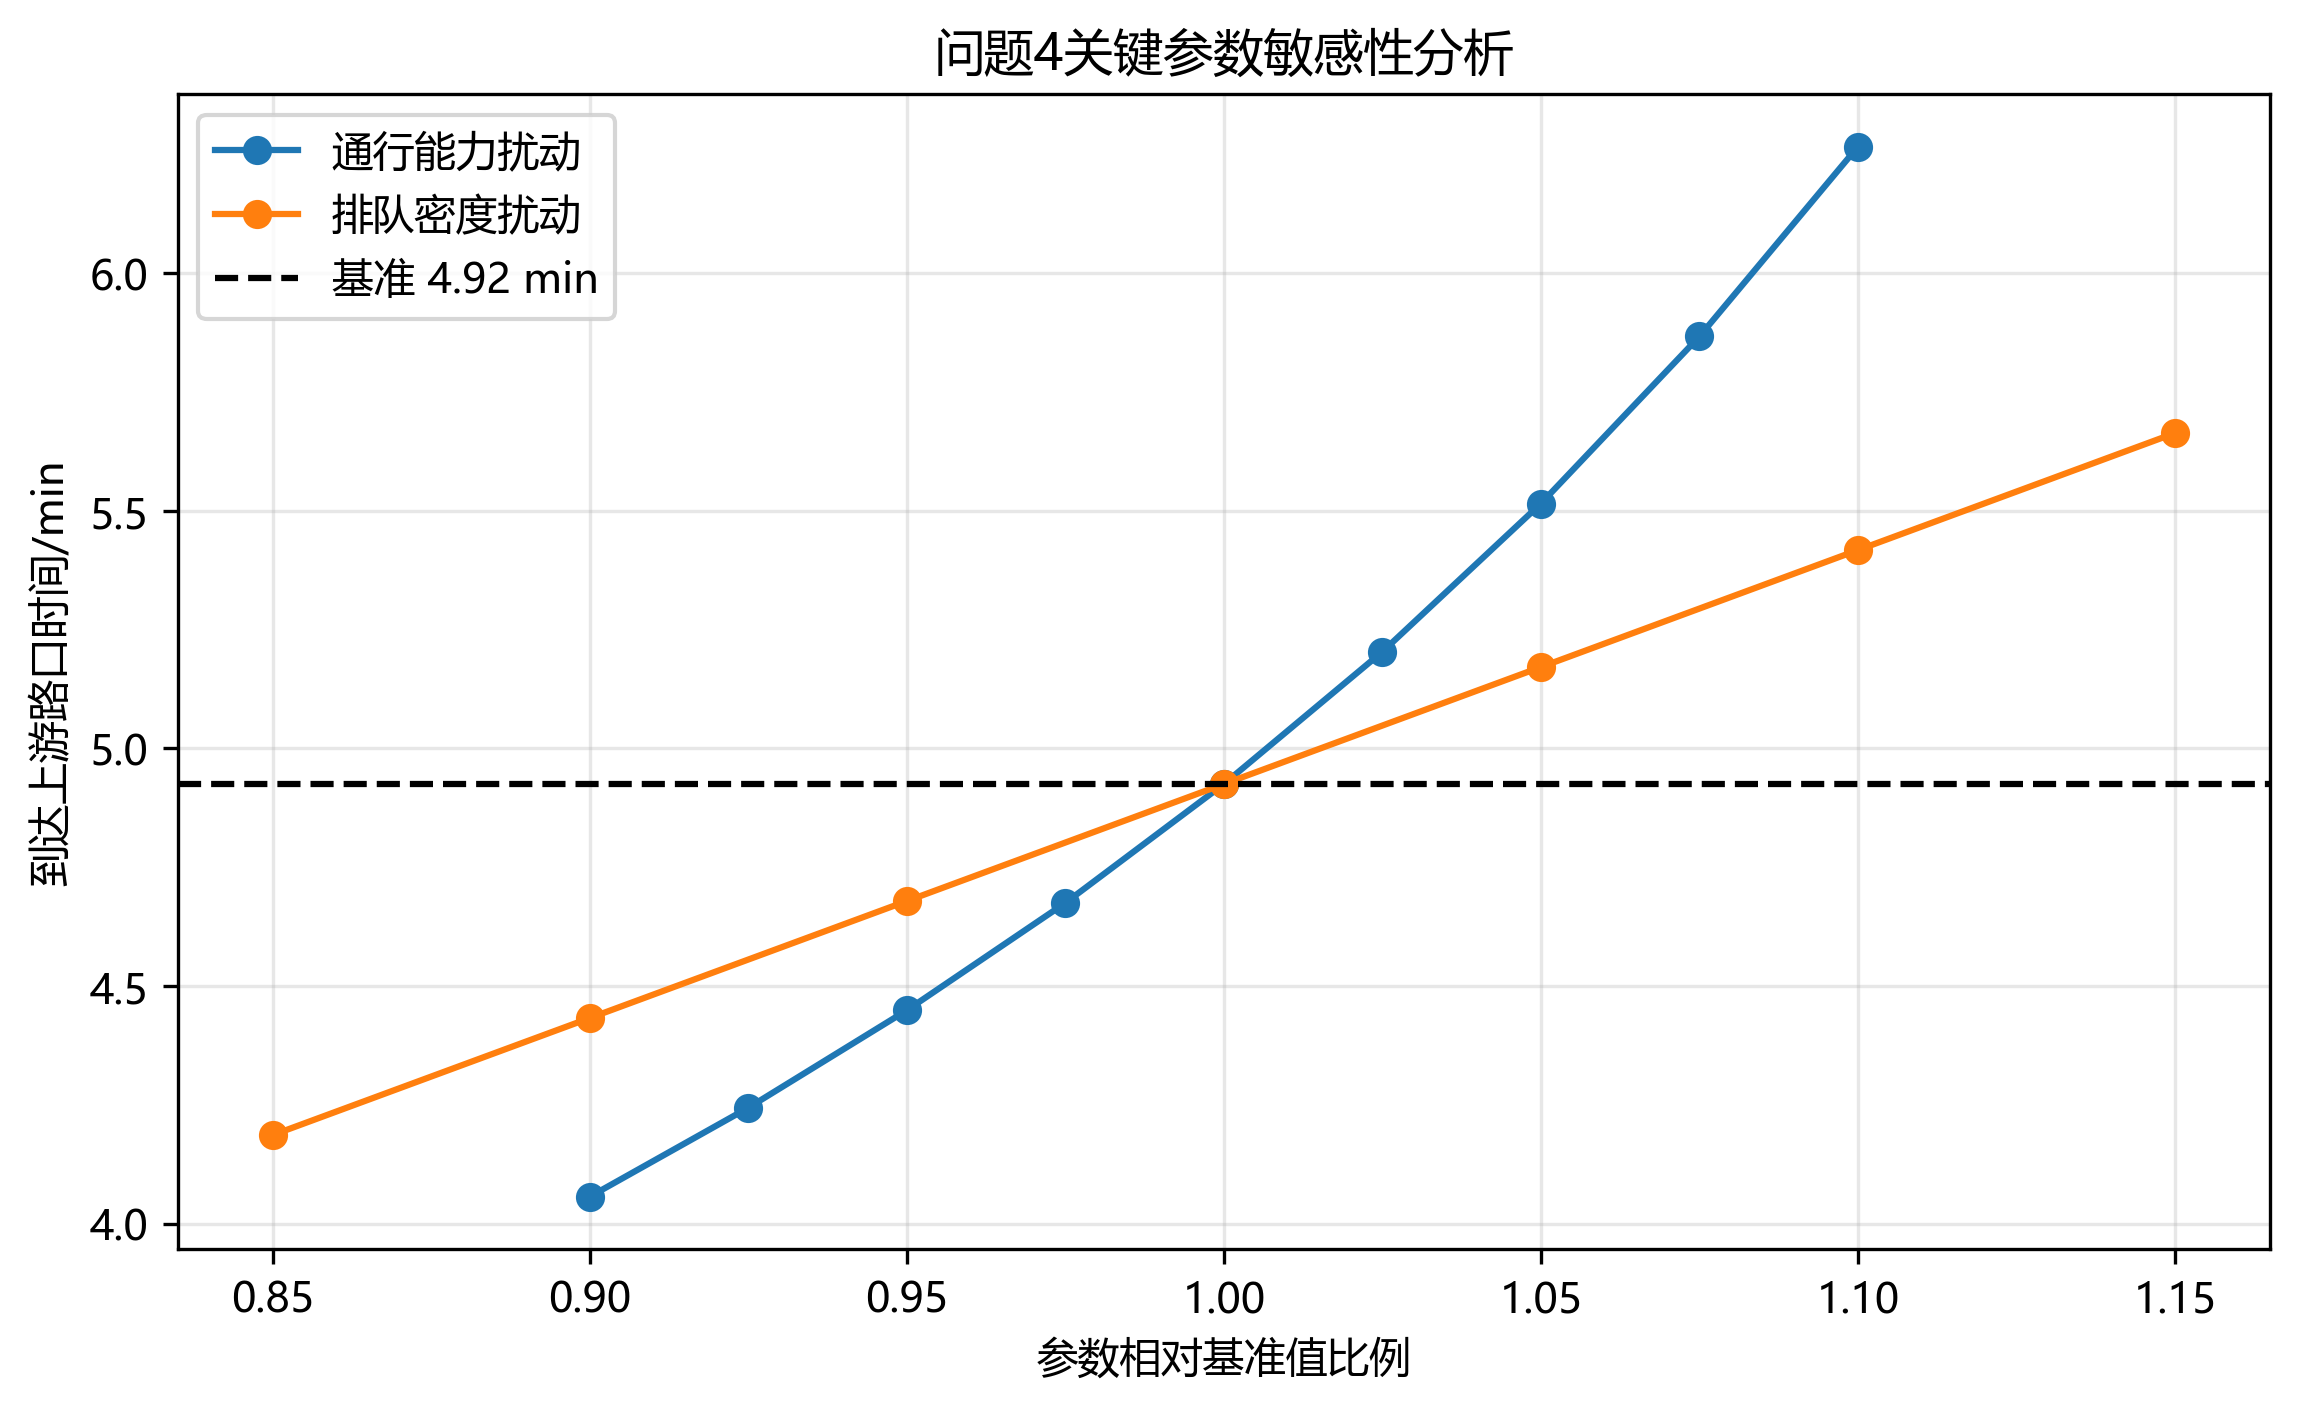
\includegraphics[width=.85\textwidth]{../quest4/figures/q4_sensitivity.png}
\caption{问题四关键参数敏感性分析}
\label{fig:q4sens}
\end{figure}

\section{模型评价、改进与推广}
\subsection{模型优点}
第一，本文模型具有清晰的交通流解释。通行能力、到达流量、排队车辆数和排队长度之间通过守恒方程相连，能够直接解释为什么事故持续时间越长、瓶颈能力越低、上游流量越大，队列越容易回溢到上游路口。相比只做经验拟合，该模型更符合交通工程机理。

第二，本文将占用车道位置纳入分析。两起事故均占用两条车道，但实际影响不同，说明按车道数简单折减会忽略横断面交通组织和换道冲突。位置修正模型虽然简洁，却能对应交通管理中的导流和占道审批决策。

第三，本文严格区分原始数据和重构数据。由于目录缺少视频附件，论文没有伪造逐帧计数，而是将数据限制写入摘要、数据审计和冻结数字文件。这使支撑材料可复现，也便于后续取得原始视频后替换数据。

\subsection{模型局限}
第一，本文使用的是参数化重构数据，无法替代真实视频的人工计数或目标检测结果。因此数值结果应理解为在合理交通流参数下的示范性估算，而不是对原视频的最终实测结论。若要用于竞赛正式提交，应补充附件视频逐分钟通过量和到达量统计。

第二，模型将排队密度设为常数，但实际排队密度会随车辆组成、驾驶员跟驰行为、车道数、车速和信号状态变化。常数密度简化便于计算，但会给问题四的到达时间带来不确定性。敏感性分析已经展示了该不确定性。

第三，回归模型采用线性形式，能够解释主要趋势，但对信号周期、非线性换道冲突和排队溢出后的路网反馈刻画不足。当队列到达上游路口后，上游交叉口放行能力和转向比例会反过来影响到达流量，需使用更复杂的元胞传输模型或微观仿真。

\subsection{改进方向}
若取得原始视频，第一步应使用人工计数或目标检测模型提取每分钟通过事故横断面和进入路段的车辆类型，按题目要求换算为标准车当量。第二步可结合附件4、附件5的上游路口渠化和信号配时，精确计算不同相位的到达流量。第三步可采用LWR冲击波模型或元胞传输模型刻画队列形成、消散和回溢过程，并用视频中实际队列长度进行校准。第四步可比较不同应急处置方案，如提前分流、临时调整信号绿信比、设置锥桶导流区等，形成可执行的交通管理建议。

\section{结论}
本文在附件视频缺失的约束下，完成了车道被占用影响城市道路通行能力的可复现建模流程。主要结论如下：
\begin{enumerate}
\item 视频1事故期间横断面实际通行能力平均为1022.4 $\pcu/h$，能力随上游信号与换道冲突波动，最小值为752.4 $\pcu/h$。
\item 不同占用车道会造成显著差异。视频2平均能力为815.6 $\pcu/h$，较视频1低20.2\%，说明占用位置会影响剩余车道有效利用率。
\item 排队长度由通行能力缺口和持续时间共同决定。多元回归 $R^2=0.873$，持续时间系数为28.176，表明快速撤离事故和恢复服务率是控制排队的关键。
\item 当事故横断面距上游路口140 m，上游流量1500 $\pcu/h$，初始排队为零且事故持续不撤离时，排队到达上游路口约需4.92 min。该时间对事故瓶颈能力和排队密度较敏感，应在事故发生后数分钟内启动上游分流和现场处置。
\end{enumerate}

\section{参考文献}
\begin{enumerate}
\item 全国大学生数学建模竞赛组委会. 2013高教社杯全国大学生数学建模竞赛A题：车道被占用对城市道路通行能力的影响[Z]. 2013.
\item 李梦圆, 陈亚男, 戴辞源, 等. 车道被占用对城市道路通行能力的影响[J]. 贵州师范学院学报, 2013(12).
\item 贾文. 车道被占用对城市道路通行能力的影响[J]. 齐鲁工业大学学报, 2014(01).
\item Transportation Research Board. Highway Capacity Manual[M]. Washington, D.C.: National Research Council, 2010.
\item May A D. Traffic Flow Fundamentals[M]. Englewood Cliffs: Prentice Hall, 1990.
\item Daganzo C F. The cell transmission model: A dynamic representation of highway traffic consistent with the hydrodynamic theory[J]. Transportation Research Part B, 1994, 28(4):269--287.
\end{enumerate}

\appendix
\section{支撑材料说明}
支撑材料目录包括：\verb|data/|保存原始题面文档，\verb|references/|保存题面提取文本和外部资料记录，\verb|quest1/|至\verb|quest4/|分别保存各问题代码、图表和输出表，\verb|results/frozen_numbers.json|保存论文关键数字，\verb|tables/final_results_summary.csv|保存最终结果摘要，\verb|run_modeling.py|为一键重现实验入口。

\section{复现命令}
\begin{verbatim}
python "<LOCAL_MATH_MODELING_TEST_ROOT>/2013年赛题/2013A/支撑材料/run_modeling.py"
cd "<LOCAL_MATH_MODELING_TEST_ROOT>/2013年赛题/2013A/支撑材料/papper"
xelatex -interaction=nonstopmode 论文.tex
xelatex -interaction=nonstopmode 论文.tex
xelatex -interaction=nonstopmode 论文.tex
\end{verbatim}

\section{三层质量审计}
L1建模合理性：通过。四个子问题均建立了题目要求与模型输出映射，假设均服务于通行能力、排队累积和情景估算模型，且包含baseline对比。L2求解正确性：有条件通过。代码可复现、随机种子固定、图表和冻结数字已生成；但由于原始视频附件缺失，视频相关数值为参数化重构而非真实计数。L3论文质量：通过。论文包含摘要关键数字、目录、模型推导、图表解释、敏感性分析、模型评价、参考文献和附录说明。
\end{document}
